% Template for PLoS
% Version 3.5 March 2018
%
% % % % % % % % % % % % % % % % % % % % % %
%
% -- IMPORTANT NOTE
%
% This template contains comments intended
% to minimize problems and delays during our production
% process. Please follow the template instructions
% whenever possible.
%
% % % % % % % % % % % % % % % % % % % % % % %
%
% Once your paper is accepted for publication,
% PLEASE REMOVE ALL TRACKED CHANGES in this file
% and leave only the final text of your manuscript.
% PLOS recommends the use of latexdiff to track changes during review, as this will help to maintain a clean tex file.
% Visit https://www.ctan.org/pkg/latexdiff?lang=en for info or contact us at latex@plos.org.
%
%
% There are no restrictions on package use within the LaTeX files except that
% no packages listed in the template may be deleted.
%
% Please do not include colors or graphics in the text.
%
% The manuscript LaTeX source should be contained within a single file (do not use \input, \externaldocument, or similar commands).
%
% % % % % % % % % % % % % % % % % % % % % % %
%
% -- FIGURES AND TABLES
%
% Please include tables/figure captions directly after the paragraph where they are first cited in the text.
%
% DO NOT INCLUDE GRAPHICS IN YOUR MANUSCRIPT
% - Figures should be uploaded separately from your manuscript file.
% - Figures generated using LaTeX should be extracted and removed from the PDF before submission.
% - Figures containing multiple panels/subfigures must be combined into one image file before submission.
% For figure citations, please use "Fig" instead of "Figure".
% See http://journals.plos.org/plosone/s/figures for PLOS figure guidelines.
%
% Tables should be cell-based and may not contain:
% - spacing/line breaks within cells to alter layout or alignment
% - do not nest tabular environments (no tabular environments within tabular environments)
% - no graphics or colored text (cell background color/shading OK)
% See http://journals.plos.org/plosone/s/tables for table guidelines.
%
% For tables that exceed the width of the text column, use the adjustwidth environment as illustrated in the example table in text below.
%
% % % % % % % % % % % % % % % % % % % % % % % %
%
% -- EQUATIONS, MATH SYMBOLS, SUBSCRIPTS, AND SUPERSCRIPTS
%
% IMPORTANT
% Below are a few tips to help format your equations and other special characters according to our specifications. For more tips to help reduce the possibility of formatting errors during conversion, please see our LaTeX guidelines at http://journals.plos.org/plosone/s/latex
%
% For inline equations, please be sure to include all portions of an equation in the math environment.
%
% Do not include text that is not math in the math environment.
%
% Please add line breaks to long display equations when possible in order to fit size of the column.
%
% For inline equations, please do not include punctuation (commas, etc) within the math environment unless this is part of the equation.
%
% When adding superscript or subscripts outside of brackets/braces, please group using {}.
%
% Do not use \cal for caligraphic font.  Instead, use \mathcal{}
%
% % % % % % % % % % % % % % % % % % % % % % % %
%
% Please contact latex@plos.org with any questions.
%
% % % % % % % % % % % % % % % % % % % % % % % %

\documentclass[10pt,letterpaper]{article}
\usepackage[top=0.85in,left=2.75in,footskip=0.75in]{geometry}

% amsmath and amssymb packages, useful for mathematical formulas and symbols
\usepackage{amsmath,amssymb}

% Use adjustwidth environment to exceed column width (see example table in text)
\usepackage{changepage}

% Use Unicode characters when possible
\usepackage[utf8x]{inputenc}

% textcomp package and marvosym package for additional characters
\usepackage{textcomp,marvosym}

% cite package, to clean up citations in the main text. Do not remove.
% \usepackage{cite}

% Use nameref to cite supporting information files (see Supporting Information section for more info)
\usepackage{nameref,hyperref}

% line numbers
\usepackage[right]{lineno}

% ligatures disabled
\usepackage{microtype}
\DisableLigatures[f]{encoding = *, family = * }

% color can be used to apply background shading to table cells only
\usepackage[table]{xcolor}

% array package and thick rules for tables
\usepackage{array}

% create "+" rule type for thick vertical lines
\newcolumntype{+}{!{\vrule width 2pt}}

% create \thickcline for thick horizontal lines of variable length
\newlength\savedwidth
\newcommand\thickcline[1]{%
  \noalign{\global\savedwidth\arrayrulewidth\global\arrayrulewidth 2pt}%
  \cline{#1}%
  \noalign{\vskip\arrayrulewidth}%
  \noalign{\global\arrayrulewidth\savedwidth}%
}

% \thickhline command for thick horizontal lines that span the table
\newcommand\thickhline{\noalign{\global\savedwidth\arrayrulewidth\global\arrayrulewidth 2pt}%
\hline
\noalign{\global\arrayrulewidth\savedwidth}}


% Remove comment for double spacing
%\usepackage{setspace}
%\doublespacing

% Text layout
\raggedright
\setlength{\parindent}{0.5cm}
\textwidth 5.25in
\textheight 8.75in

% Bold the 'Figure #' in the caption and separate it from the title/caption with a period
% Captions will be left justified
\usepackage[aboveskip=1pt,labelfont=bf,labelsep=period,justification=raggedright,singlelinecheck=off]{caption}
\renewcommand{\figurename}{Fig}

% Use the PLoS provided BiBTeX style
% \bibliographystyle{plos2015}

% Remove brackets from numbering in List of References
\makeatletter
\renewcommand{\@biblabel}[1]{\quad#1.}
\makeatother



% Header and Footer with logo
\usepackage{lastpage,fancyhdr,graphicx}
\usepackage{epstopdf}
%\pagestyle{myheadings}
\pagestyle{fancy}
\fancyhf{}
%\setlength{\headheight}{27.023pt}
%\lhead{
\includegraphics[width=2.0in]{PLOS-submission.eps}}
\rfoot{\thepage/\pageref{LastPage}}
\renewcommand{\headrulewidth}{0pt}
\renewcommand{\footrule}{\hrule height 2pt \vspace{2mm}}
\fancyheadoffset[L]{2.25in}
\fancyfootoffset[L]{2.25in}
\lfoot{\today}

%% Include all macros below

\newcommand{\lorem}{{\bf LOREM}}
\newcommand{\ipsum}{{\bf IPSUM}}





\usepackage{forarray}
\usepackage{xstring}
\newcommand{\getIndex}[2]{
  \ForEach{,}{\IfEq{#1}{\thislevelitem}{\number\thislevelcount\ExitForEach}{}}{#2}
}

\setcounter{secnumdepth}{0}

\newcommand{\getAff}[1]{
  \getIndex{#1}{Smith College}
}

\providecommand{\tightlist}{%
  \setlength{\itemsep}{0pt}\setlength{\parskip}{0pt}}

\begin{document}
\vspace*{0.2in}

% Title must be 250 characters or less.
\begin{flushleft}
{\Large
\textbf\newline{The Graphical Analysis on the Gap between Supply and Demand for Early Ed
Childcare Services} % Please use "sentence case" for title and headings (capitalize only the first word in a title (or heading), the first word in a subtitle (or subheading), and any proper nouns).
}
\newline
% Insert author names, affiliations and corresponding author email (do not include titles, positions, or degrees).
\\
Jocelyn Hu\textsuperscript{\getAff{Smith College}},
Kat Kyuchukova\textsuperscript{\getAff{Smith College}},
Paige Patrick\textsuperscript{\getAff{Smith College}}\\
\bigskip
\textbf{\getAff{Smith College}}SDS, 1 Chapin Way, Northampton, MA 01063\\
\bigskip
\end{flushleft}
% Please keep the abstract below 300 words
\section*{Abstract}
Community Labor United is a non-profit organization that is currently
working to investigate the negligence in childcare provision for low and
middle-income families within the Greater Boston Area, in order to
promote reforms within the current system provided by the Department of
Early Education and Care. Using interactive maps, the research outlined
in this paper highlights two gaps in the current childcare structure.
The first being how the hours that early education childcare providers
keep do not support families that work primarily nonstandard schedules.
The second being how the number of slots for early education provision
does not align with the number of children age five and under that live
within each neighborhood and census tract. The interaction between these
two gaps drastically impacts the livelihood of working class families
and it is our hope that this research will provide evidence that the
current system in place needs to be reconstructed, in order to support
all households in Massachusetts.

% Please keep the Author Summary between 150 and 200 words
% Use first person. PLOS ONE authors please skip this step.
% Author Summary not valid for PLOS ONE submissions.

\linenumbers

% Use "Eq" instead of "Equation" for equation citations.
\section{Introduction}\label{introduction}

\subsection{Community Labor United}\label{community-labor-united}

Community Labor United (CLU) is a non-profit organization, operating in
the Greater Boston Area, that works with other community-based
establishments and labor unions across Massachusetts to cultivate
strategic campaigns that protect and promote the interests of low and
middle-income working class families {[}1{]}. Their overall goal is to
promote policies that advocate for accessible jobs, healthcare,
childcare, housing and environmental justice for working class
households {[}1{]}. Through their \emph{Our Care That Works} coalition
that launched publicly this year, Community Labor United aims to bring
together various local cooperative groups to confront the child care
crisis in Massachusetts. More specific to this research, CLU is
interested in examining the inconsistencies in childcare within the
Greater Boston Area, caused by the negligence of the Department of Early
Education and Care (EEC). This investigative exploration into childcare
provision gaps within the Greater Boston Area will allow Community Labor
United to communicate to the EEC the demand for the standardization of
childcare within Massachusetts.

\subsection{EEC Literature Review}\label{eec-literature-review}

``The ethical imperative of a society to support the care of inevitable
dependents makes care a social responsibility and therefore creates an
important role for the state'' (p.~150) {[}2{]}. The Department of Early
Education and Care's mission is to maintain the growth and development
of all children, by providing quality childcare programs and resources
for families within their communities {[}3{]}. However, the research led
by Community Labor United and their affiliated organizations shows that
the EEC has been unable to effectively execute their commitment for low
and middle-income working class families {[}1{]}. The reason CLU's
attention is on low and middle-income families is because more than five
million Americans are not only scheduled for fewer hours, days, or weeks
than they prefer working, but the daily timing of their work schedules
can often be irregular or unpredictable {[}4{]}. According to the
General Social Survey obtained by the Economic Policy Institute, the
lowest income workers typically face the most irregular work schedules
{[}4{]}. As contemporary research shows, having a fluctuating and
unpredictable work schedule puts working-class families at a
disadvantage to finding accessible, reliable childcare {[}5{]}.

One of the biggest hurdles to researching the impact nonstandard hours
have on the livelihood of low and middle-income families, is that the
existing measures in national data sets do not capture multiple
dimensions of work schedules {[}5{]}. This makes it difficult to
accurately assess the number of families that are working outside the
``typical'' 9am - 5pm office job. In turn, this hinders the ability for
researchers and advocates to highlight the need for childcare reform, to
include operating hours that accommodate more nonstandard schedules.
There should be additional items on national surveys that gather
information on divergence from the ``typical'' work arrangement to make
it possible to examine fluctuations in work schedule timing and hours
{[}5{]}. However, until national data sets are able to reflect more
inclusive and diverse lifestyles, research conducted to help highlight
the needs of families who work nonstandard hours will remain difficult
to gather and interpret {[}5{]}.

There is a need for focus on understanding the childcare needs of low
and middle-income families, in order to address the pressing social
problems of our time surrounding inadequate provision of quality care to
the elderly, children, and those who are ill or disabled {[}2{]}. More
specifically, projects should include completing empirical mapping of
childcare, to provide a bridge between the goals of care theorists and
the specific policy context of care in a given local area {[}2{]}.
Paired with an accurate representation of the childcare demands of the
community, mapping the current childcare supply will allow the
opportunity to understand the gaps in the current childcare system
provided by the Department of Early Education and Care in hopes the
state supports more consistent and accurate policy implementations
{[}6{]}.

\subsection{Research Question}\label{research-question}

As noted above, the general goal for this research is to examine the
inconsistencies in the EEC by highlighting childcare provision gaps in
the Greater Boston Area. More specifically, this project focuses on
illustrating a disparity in operating hours and capacity for childcare
providers on the neighborhood level and census tract level. Because
Community Labor United is concentrated on understanding how the low and
middle-income households are impacted by the current childcare system,
our project emphasizes the childcare demands needed for working class
families. Additionally, CLU is interested in concentrating on early
education provision care, which encompasses childcare for children ages
five and under. For operating hours, we look at how the non-typical work
week is affected by the early education provision that is currently
supplied, since people with low and middle-incomes work at times that
operate outside the typical 9:00am - 5:00pm job. We want to understand
if there were a sufficient number of childcare facilities that could
offer early education provision outside Monday - Friday, 7:30am -
6:00pm, for people in the Greater Boston Area. Similarly for capacity,
we want to highlight the lack of available slots for early education
provision for working households with children age five and under. This
is because working-class families typically have all parents in the
household in the workforce, so it is crucial that the childcare capacity
supply matches the demand.

Individually, the child provision gaps in hours and capacity shows how
the Department of Early Education and Care has neglected low and
middle-income families in specific ways. However, we also think it's
important to understand how the interaction between lack of available
childcare hours and lack of early education provision spots impact these
households overall. To best convey that interaction, we have compiled
our visualizations and supporting information on an easily accessible
platform. This allows for the user to quickly navigate the various maps
for hours and capacity, and also share these findings with all
appropriate parties. It is our hope that Community Labor United will be
able to use the visualizations we've created to motivate the Department
of Early Education to make reforms to the current childcare system to be
more accommodating for all families in Massachusetts, regardless of
occupation or availability.

\section{Method}\label{method}

In order to quantify the gap in supply and demand for childcare in
Boston, we focus on the capacity of the existing childcare providers in
comparison to the number of children who need childcare, as well as the
hours that providers are able to provide childcare in comparison to the
hours when childcare is most needed by those who work outside standard
hours. We focus on these areas both for their urgency in affecting
access to and need for childcare, as well as for the lack of existing
research that exists on the gaps between the childcare that exists and
the childcare that is needed.

\subsection{Data}\label{data}

The data from our main analyses consists of two data sources, one
addressing the supply side of the gaps in childcare, and the other
addressing the demand. The supply data source comes from \emph{Community
Labor United}, and it is a collection of providers from the Department
of Early Education and Care (EEC) in Massachusetts. The initial dataset
consists of 8,318 observations, with each row representing a childcare
provider in Massachusetts. Since our project focuses specifically on the
Boston area, we filtered the dataset to contain only neighborhoods in
Boston. leaves us with 764 remaining childcare providers. We include 13
neighborhoods: Allston, Boston, South Boston, Brighton, Charlestown,
Dorchester, East Boston, Hyde Park, Jamaica Plain, Mattapan, Roslindale,
Roxbury, and West Roxbury. Neighborhoods with the highest number of
providers include central Boston (100), Dorchester (203) and Roxbury
(70).

There is no existing dataset that tells us about childcare demand
specifically, so to answer this question we use census data,
specifically the \emph{American Community Survey} (ACS), and filter for
certain variables of interest. The following methodology will discuss
specific variables in detail, but all data is derived from the 2016
American Community Survey and is filtered for Suffolk County,
Massachusetts.

We want to convey the gap in childcare by a geography that is big enough
to generalize our conclusions , but small enough so that we don't
overlook any areas that might have findings of interest. Through
consultation with CLU's Senior Researcher, here we convey our results by
the neighborhood level. To do this, we access Boston neighborhood
shapefile data {[}7{]} and assign each EEC childcare provider to a
certain neighborhood. Since the census data of interest is only
accessible by tract, we develop a file that matches each census tract to
a neighborhood, and includes both tract geometry and neighborhood
geometry to allow for easy mapping. More about this process is discussed
in the challenges section.

\section{Capacity}\label{capacity}

\subsection{Supply}\label{supply}

To get a sense of the slots available for early education provision, we
take the EEC dataset and filter only for providers that provide early
education childcare. We use the tidyverse package {[}8{]} to group the
providers by census tract, and calculated the total number of slots for
early education childcare in each tract. Since we are interested in
looking at differences on both the tract level and the neighborhood
level, we repeat this process for neighborhood so that we also have the
total number of slots for early education childcare in each
neighborhood. We merge these datasets with the respective geometry for
each geography, to allow us to map the results.

\subsection{Demand}\label{demand}

Demand for capacity of childcare is assessed through the use of the 2016
ACS. The tigris and tidycensus {[}9,10{]} packages are used in
congruence with an API key, in order to access census data in R. We use
the American Community Survey, as opposed to other forms of census data,
because it is the only survey that is easily compatible with R.
Additionally, it also has data available for all variables of interest
on the tract level for Suffolk County.

To quantify the number of children that need childcare, we use the ACS
variable ``B23008'', which gives estimates per tract of the number of
children under 6 in two-parent households with both parents in the labor
force, as well as single parent households (either mother or a father)
with the parent in the labor force. We then add up these variables, with
the assumption that anybody with all parents in the labor force would
need childcare. See Table 1 for descriptive statistics. To get a
percentage of children under 6 with all parents in the labor force, we
divide this number by the total number of children under 6. All
calculations are per tract.

\begin{table}[!h]
\centering\begingroup\fontsize{10}{12}\selectfont

\begin{tabular}{l|r|r|r|r|r}
\hline
\multicolumn{6}{c|}{Table 1: Working Force Children Demand Summary Statistics} \\
\cline{1-6}
  & n & mean & sd & min & max\\
\hline
\rowcolor{gray!6}  Count Children Under 6 & 204 & 175.83 & 142 & 0 & 700\\
\hline
\end{tabular}
\endgroup{}
\end{table}

\subsection{Maps}\label{maps}

Three maps are made as a final product for visualizing the gap in
capacity. Two of these maps (Figure 1 and Figure 2) look at supply and
demand at the tract level. The first is mapping the raw number of
children under 6 with all parents in the workforce, while the second
shows the raw number of slots available for early education care per
tract. This allows for the supply and demand side of capacity to be
easily compared to one another. The third map (Figure 3) quantifies the
difference in supply and demand by neighborhood, as a ratio of children
to childcare slots. We create this ratio by dividing the number of
children under 6 with working parents by the number of childcare slots
available. We created this ratio based on the Center for American
Progress' definition of a childcare desert, which says that in any
census tract with over 50 children under age five, a ratio of over 3:1
of children to childcare slots classifies that census tract as a
childcare desert {[}11{]}. However, this definition is by census tract.
Since it is unrealistic that one would restrict their childcare search
to within their census tract, a rather small boundary, we want to give a
more realistic range of how far a childcare search might go, hence our
rationale for grouping by neighborhood.

\begin{figure}

{\centering 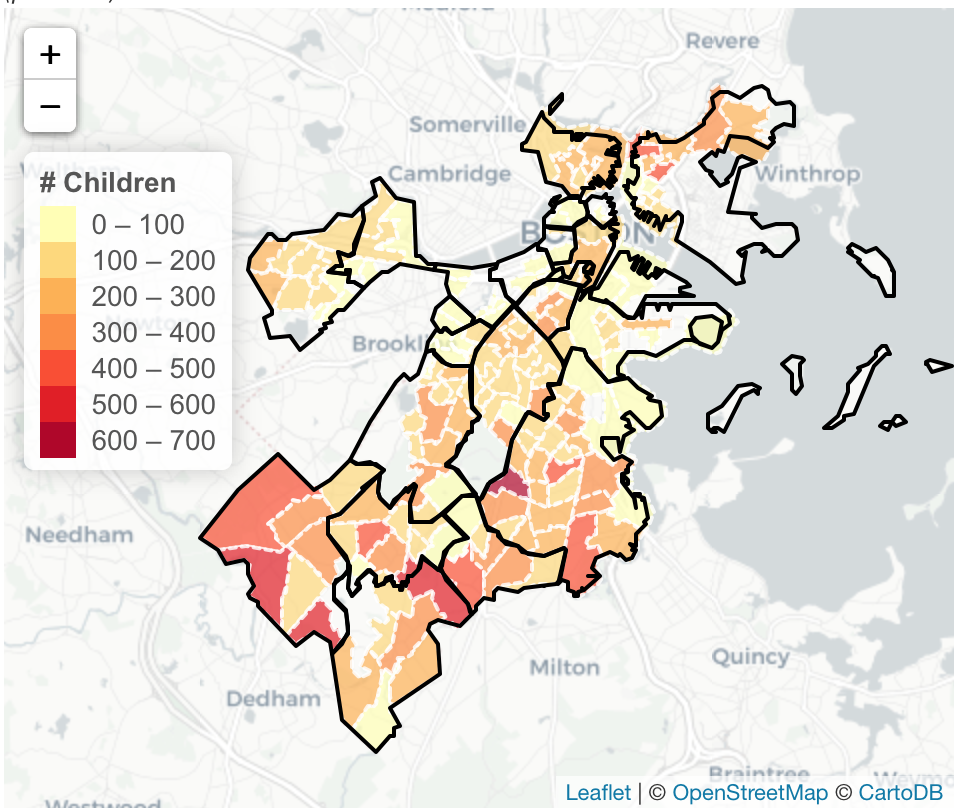
\includegraphics[width=0.8\linewidth]{fig1_capacitytractdemand} 

}

\caption{Number of children under 6 from working families}\label{fig:unnamed-chunk-4}
\end{figure}

\begin{figure}

{\centering 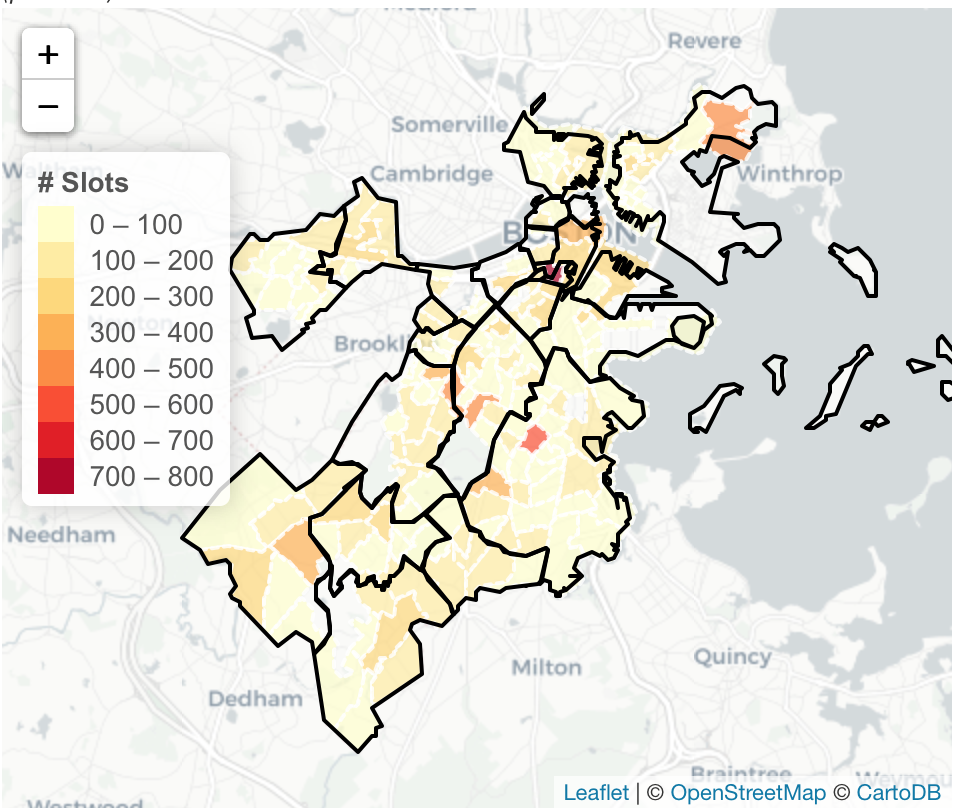
\includegraphics[width=0.8\linewidth]{fig2_capacitytractsupply} 

}

\caption{Number of slots available for early ed by tracts}\label{fig:unnamed-chunk-5}
\end{figure}

\begin{figure}

{\centering 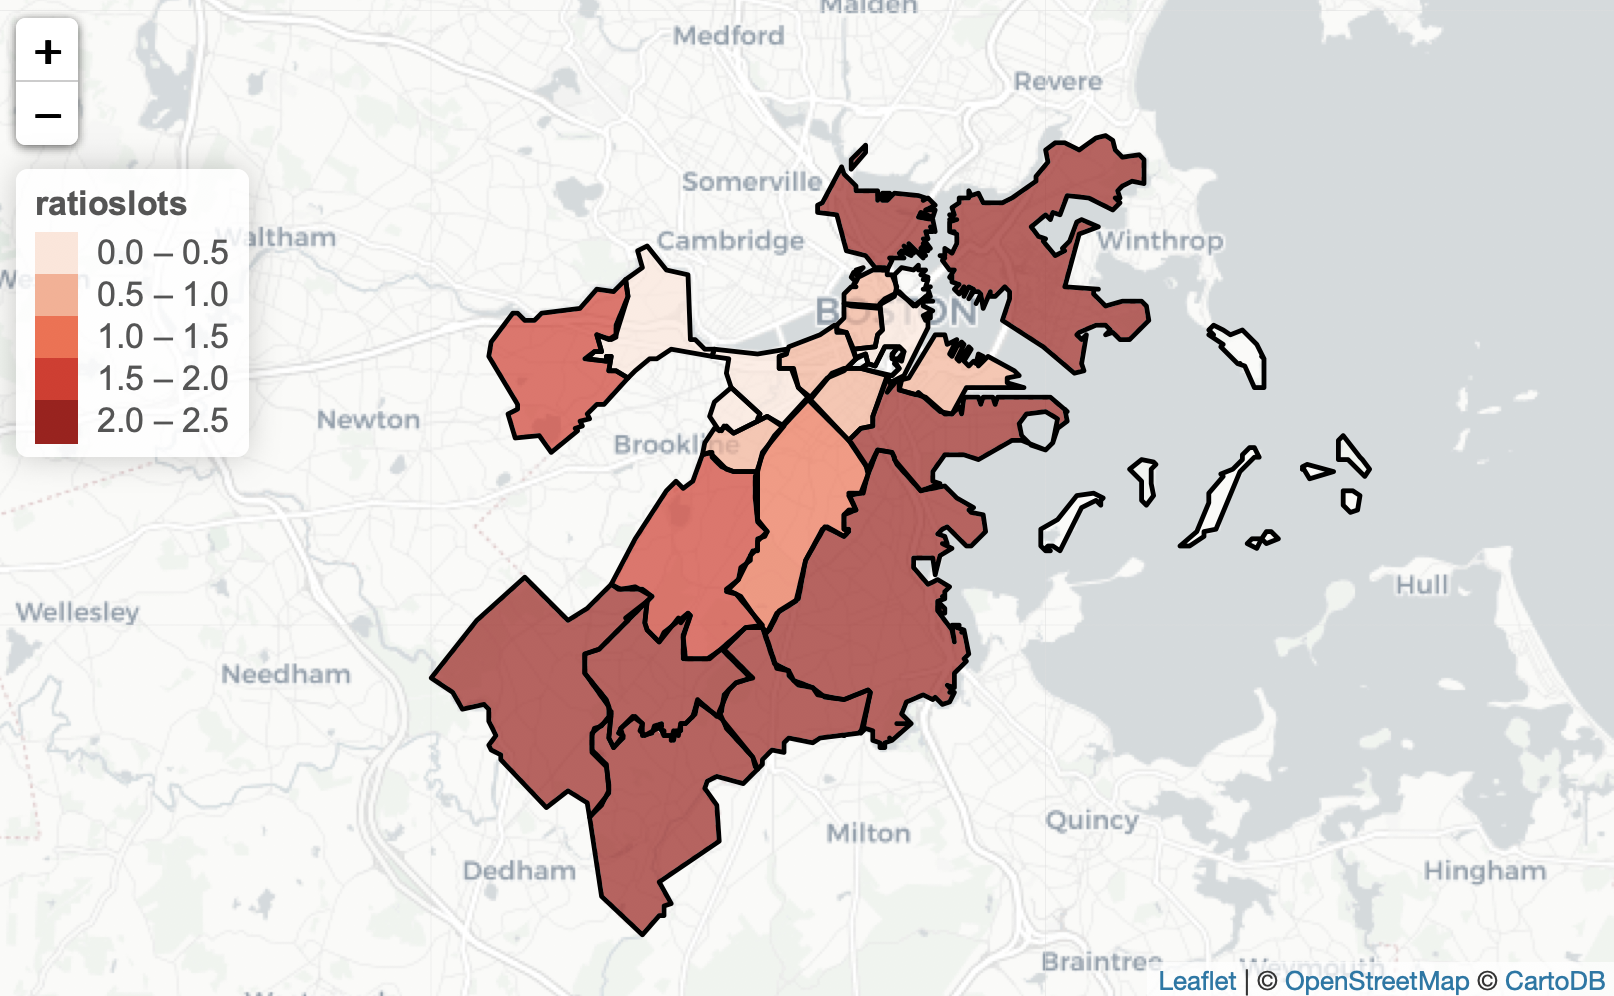
\includegraphics[width=1\linewidth]{fig3} 

}

\caption{Ratio of children under 6 from working families to slots}\label{fig:unnamed-chunk-6}
\end{figure}

\section{Hours}\label{hours}

\subsection{Supply}\label{supply-1}

Our main focus with the question of hours was to get a sense of the
providers who provide childcare outside of the typical standard workday,
which we define as anytime outside of 7:30am-6pm on weekdays
(\emph{CLU}). We did not include weekday care since there are only a few
providers that provide any weekend care at all. Therefore, to get our
dataset for supply, we create a variable based on the information about
hours in the EEC dataset to flag any provider that provided care during
nonstandard hours, and summarize the number of slots they had for those
hours.

\subsection{Demand}\label{demand-1}

One large problem with census data is that in any workday related
variables, it assumes workers work 5 days a week, with the same number
of hours every day. This definition contradicts the purpose of our
study, which is to investigate the resources available to those who work
nonstandard hours. Therefore, the only census variable that we find
appropriate to use when investigating hours is the time leaving work.
Using previous ACS methodology given to us by CLU, we split the
nonstandard times leaving for work into three categories: early mornings
if they leave for work anytime between 12am-6:29am, evenings if they
leave for work anytime between 11am-3:59pm, late evening/overnight if
they leave for work anytime between 4pm-11:59pm. We use the ACS
variables corresponding to these responses in variable B08302, and
divide the number of people in each category by the total number of
people in the workforce to get a percentage of people in each category.
We also summarize the number of people in the three nonstandard time
chunks to get a total percentage of people leaving during any
nonstandard hour. See Table 2 for descriptive statistics.

\begin{table}[!h]
\centering\begingroup\fontsize{10}{12}\selectfont

\begin{tabular}{l|r|r|r|r|r}
\hline
\multicolumn{6}{c|}{Table 2: Hours Demand Summary Statistics} \\
\cline{1-6}
  & n & mean & sd & min & max\\
\hline
\rowcolor{gray!6}  Count Early Morning Shifts & 198 & 336.56 & 263.18 & 0 & 1270.00\\
\hline
Count Evening Shifts & 198 & 191.21 & 147.10 & 0 & 772.00\\
\hline
\rowcolor{gray!6}  Count Overnight Shifts & 198 & 129.31 & 94.41 & 0 & 505.00\\
\hline
Percent Early Morning & 198 & 16.38 & 9.40 & 0 & 67.61\\
\hline
\rowcolor{gray!6}  Percent Evening & 198 & 9.92 & 7.19 & 0 & 54.10\\
\hline
\end{tabular}
\endgroup{}
\end{table}

\subsection{Maps}\label{maps-1}

There are five maps which visualize the gap in supply and demand for
hours. Three of the maps are choropleth maps by tract visualizing the
percentage of people who leave for work at each of the nonstandard
times: early, evening, and late evening/overnight. We present a similar
map by tract using the aggregate percentage of all people leaving during
any of these nonstandard hours. Finally, to visualize supply, we present
a map of the number of slots available for nonstandard hours of
childcare by provider by tract.

\section{Results}\label{results}

In this section we summarize the data used and how the maps we create to
illustrate the gap between demand and supply of childcare services for
children under six in the Greater Boston Area. We start by presenting
the summary statistics of the data sets, analyzing each individual map,
and then proceed to analyze the relationships between them.

\subsection{Summary Statistics}\label{summary-statistics}

\begin{table}[!h]
\centering\begingroup\fontsize{10}{12}\selectfont

\begin{tabular}{l|r|r|r|r|r}
\hline
\multicolumn{6}{c|}{Table3: \#slots for early ed (unit: slot)} \\
\cline{1-6}
  & N.Valid & Mean & Std.Dev & Min & Max\\
\hline
\rowcolor{gray!6}  \#slots by neighborhood & 811 & 1668.93 & 1063.58 & 6 & 3430\\
\hline
\#slots by providers & 811 & 25.45 & 36.37 & 3 & 325\\
\hline
\rowcolor{gray!6}  \#slots by tract & 811 & 210.26 & 200.29 & 6 & 1014\\
\hline
\end{tabular}
\endgroup{}
\end{table}

Table 3 presents the summary statistics of the number of slots available
for children under six, which is what we use to quantify the supply of
early education childcare service in the Greater Boston area. The
average capacity of a single provider in this area is 24.7 slots. The
average capacity of a neighborhood in total is 1669 slots, and the
average capacity per tract is 210 slots.

\begin{table}[!h]
\centering\begingroup\fontsize{10}{12}\selectfont

\begin{tabular}{l|r|r|r|r|r}
\hline
\multicolumn{6}{c|}{Table4: Weekdays nonstandard-hour \#slots for early ed (unit: slot)} \\
\cline{1-6}
  & N.Valid & Mean & Std.Dev & Min & Max\\
\hline
\rowcolor{gray!6}  \#off-hour slots by neighborhood & 17 & 41.18 & 39.86 & 8 & 140\\
\hline
\#off-hour slots by providers & 17 & 26.35 & 35.45 & 6 & 140\\
\hline
\rowcolor{gray!6}  \#off-hour slots by tract & 17 & 26.35 & 35.45 & 6 & 140\\
\hline
\end{tabular}
\endgroup{}
\end{table}

Table 4 presents the summary statistics of the number of slots available
for children under six during nonstandard hours (i.e., 6pm-7:30am) on
weekdays, which is what we use to quantify the supply of off-hour early
education childcare service in the Greater Boston area. The average
off-hour capacity of a single provider is 26 slots, per neighborhood in
Boston is 41 slots, and per tract in Boston is 26 slots.

\subsection{Graphs for Capacity}\label{graphs-for-capacity}

In this section we conduct graphical analysis on our variables of
interest: capacity and hours.

Figure 1 shows the total number of children under six of whom at least
one parent is in the labor force (i.e., actively looking for or having a
job) in each tract of the Greater Boston area, which is how we quantify
the demand of early ed childcare service. We are especially interested
in this population group since they are target consumers of childcare
services for early education. The more children with parents in the
labor force indicates a higher demand for childcare. According to this
map, the tracts that have the largest number of children who might need
childcare are mainly located in East Boston, West Roxbury, Hyde Park,
and Dorchester.

Figure 2 shows a map of the number of childcare slots available for
children under six on the level of tracts, which is how we quantify the
supply of childcare service for children under six. The tracts that
contain more slots are located in East Boston, Downtown Boston, and
Dorchester, but compared to the map showing demand, the slots are more
evenly distributed across tracts. We note that providers in the east and
west parts of Boston where there is a large number of children under six
with one parent in the labor force, do not offer enough number of slots
to fulfill the need of working families in these areas. The difference
between supply and demand explains the high ratio of children that might
need childcare to slots available in these neighborhoods as shown in
Figure 3.

Figure 3 shows the ratio of children under age five to the cumulative
child care capacity in the neighborhoods of Boston. The higher the
ratio, the more children are competing to obtain a licensed child care
slot, and therefore the harder it is for a child in the neighborhood to
obtain the childcare service they need. Conversely, the less children
are competing to obtain a licensed child care slot the easier it is for
a child in the neighborhood to obtain the childcare service they need.

\begin{figure}

{\centering \includegraphics[width=0.8\linewidth]{income} 

}

\caption{Bar chart of income level and ratio of children to slots}\label{fig:unnamed-chunk-10}
\end{figure}

To more closely analyze the ratio map, we present a bar chart which
ranks the neighborhoods by the childcare ratio as shown in the Figure 4.
The chart shows that no neighborhood achieves 1:1 target ratio--mostare
facing a surplus or deficit of early ed childcare services. Secondly,
the bar chart indicates that West Roxbury, East Boston, South Boston,
Roslindale, and Dorchester have the highest ratio and therefore are
facing the most insufficient supply of early education childcare
services. Although the relationship between the gap in childcare
availability and income was not the focus of this project, one
explanation for this could be income. For example, South Boston
Waterfront has a good ratio of .3 children to every one slot, meaning
there is a surplus of childcare slots, and an average annual income of
approximately \$138,545. East Boston on the other hand has a ratio of
2.1 children to every 1 childcare slot, meaning there is a deficit of
slots, and an average income of \$52,008. As seen in Table\_\_, there
appears to be a negative relationship between average income and ratio
of children to slots. This indicates an area to be explored in the
future.

\subsection{Graphs for Hours}\label{graphs-for-hours}

In addition to the capacity variables, we also visualize the gap between
supply and demand through the hours variable, since irregular working
hours is one of the main issues faced by low-income working parents. In
this section, we look into the working hours of families and the
operating hours of providers to examine whether there is a mismatch.

\begin{figure}

{\centering 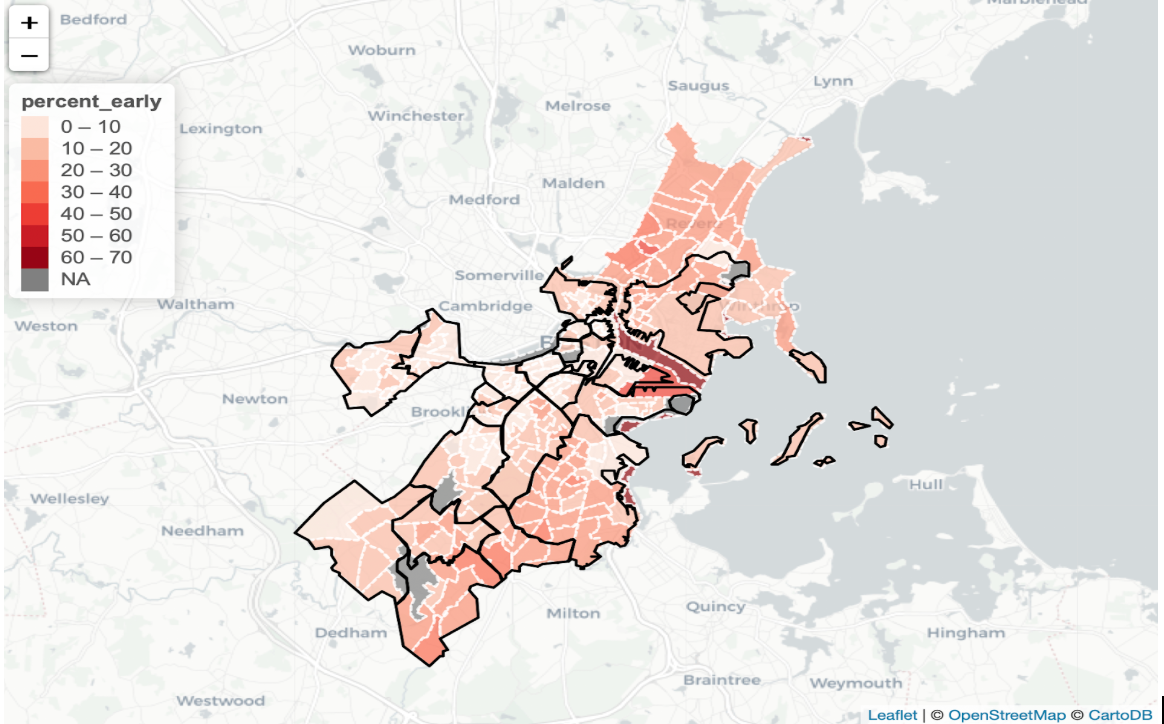
\includegraphics[width=1\linewidth]{fig4} 

}

\caption{Percentage of people that depart to work in the early morning by tract}\label{fig:unnamed-chunk-11}
\end{figure}

Figure 5 shows the percentage of parents in tracts who depart for
workplaces 12:00am to 6:59am in the early morning. On average, people
who live in the East Boston and West Boston leave earlier for work than
people who live in other regions. These are also the regions where there
are relatively larger number of children under six in need of childcare
services as shown in in figure 3. Specifically, the tracts where the
largest percentages of people leave for jobs early are located at are
waterfront areas of South Boston and Dorchester.

\begin{figure}

{\centering 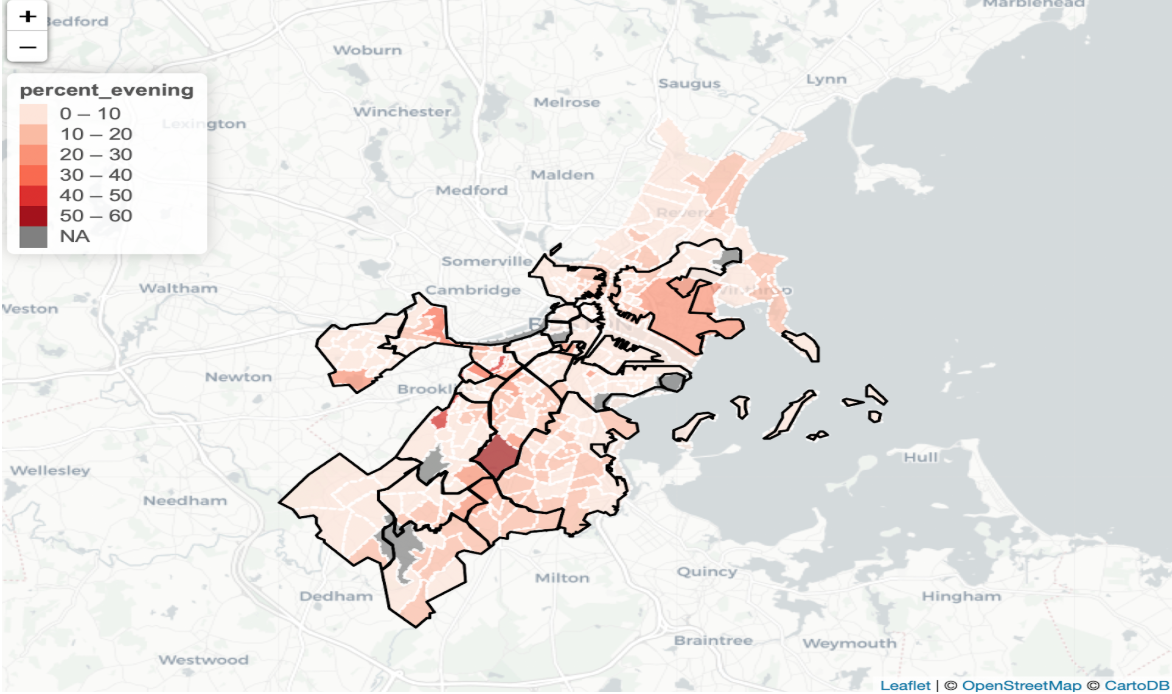
\includegraphics[width=1\linewidth]{fig5} 

}

\caption{Percentage of people that depart to work in the early evening by tract}\label{fig:unnamed-chunk-12}
\end{figure}

Figure 6 shows the percentage of people in tracts who leave for work in
the early evening between 11:00am and 3:59pm. On average, the number of
parents in East Boston, West Boston , and waterfront tracts of Brighton
and Allston that leave for work during this period of time is more than
in other areas. The tracts where the largest percentages of people leave
for work during this time period are located at Roxbury and the
waterfront areas of Jamaica Plain.

\begin{figure}

{\centering 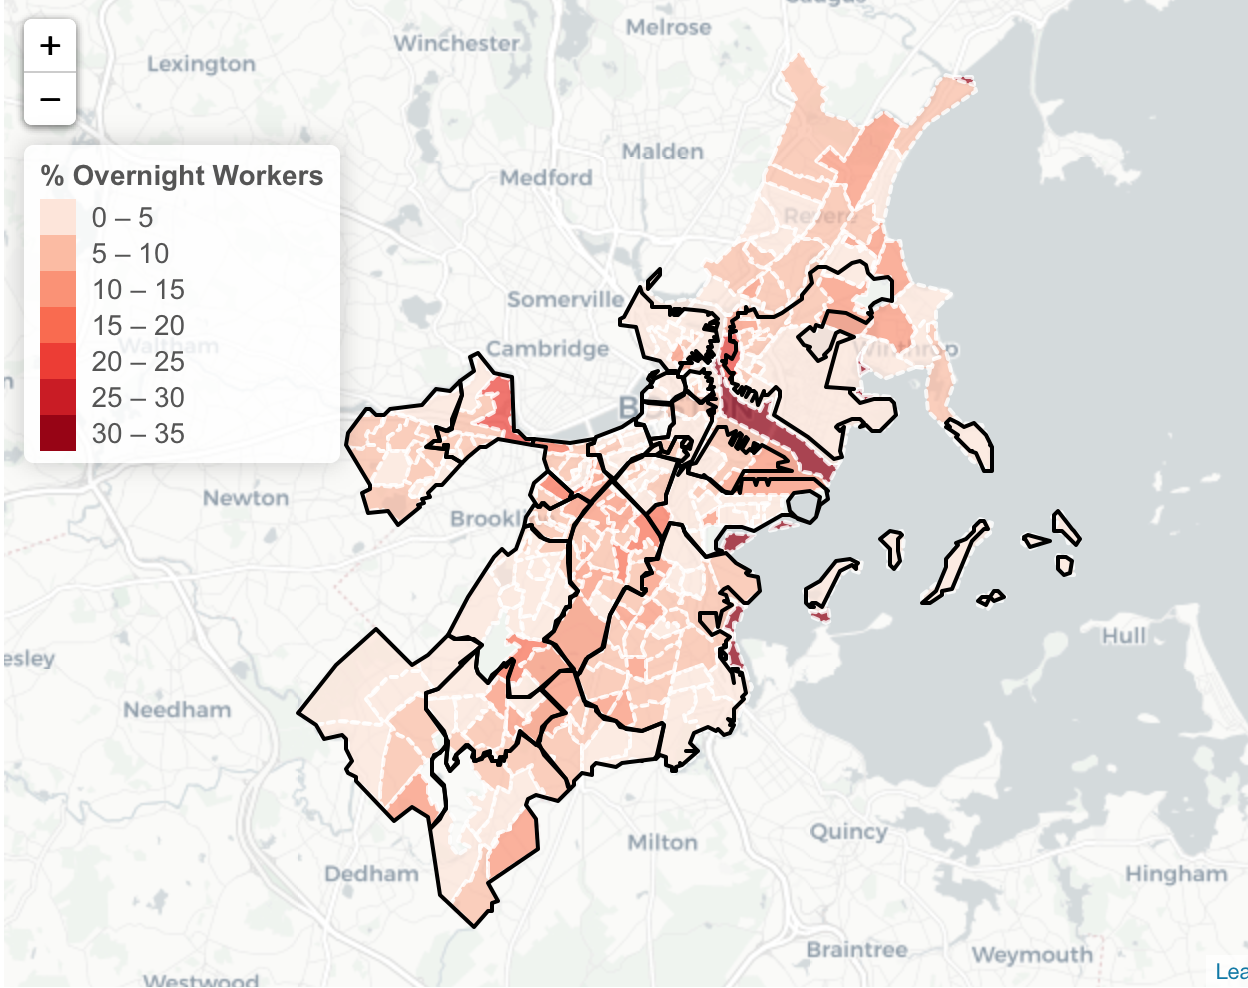
\includegraphics[width=0.8\linewidth]{fig6_percent_overnight} 

}

\caption{Percentage of people who depart to work overnight by tract}\label{fig:unnamed-chunk-13}
\end{figure}

Figure 7 shows the percentage of people in tracts who leave for work
between the hours of 4:00pm-11:59pm, who we refer to as people that work
late evening/overnight shifts. On average, people who live in downtown
Boston, West Boston, and South Boston leave later for workplaces than
people who live in other regions. These are also the regions where a
larger percentage of people leave early and where there are a relatively
larger number of children under 6 in need of childcare services.
However, the tracts where the largest percentages of people leave for
jobs overnight are located in waterfront areas of South Boston and
Dorchester.

\begin{figure}

{\centering 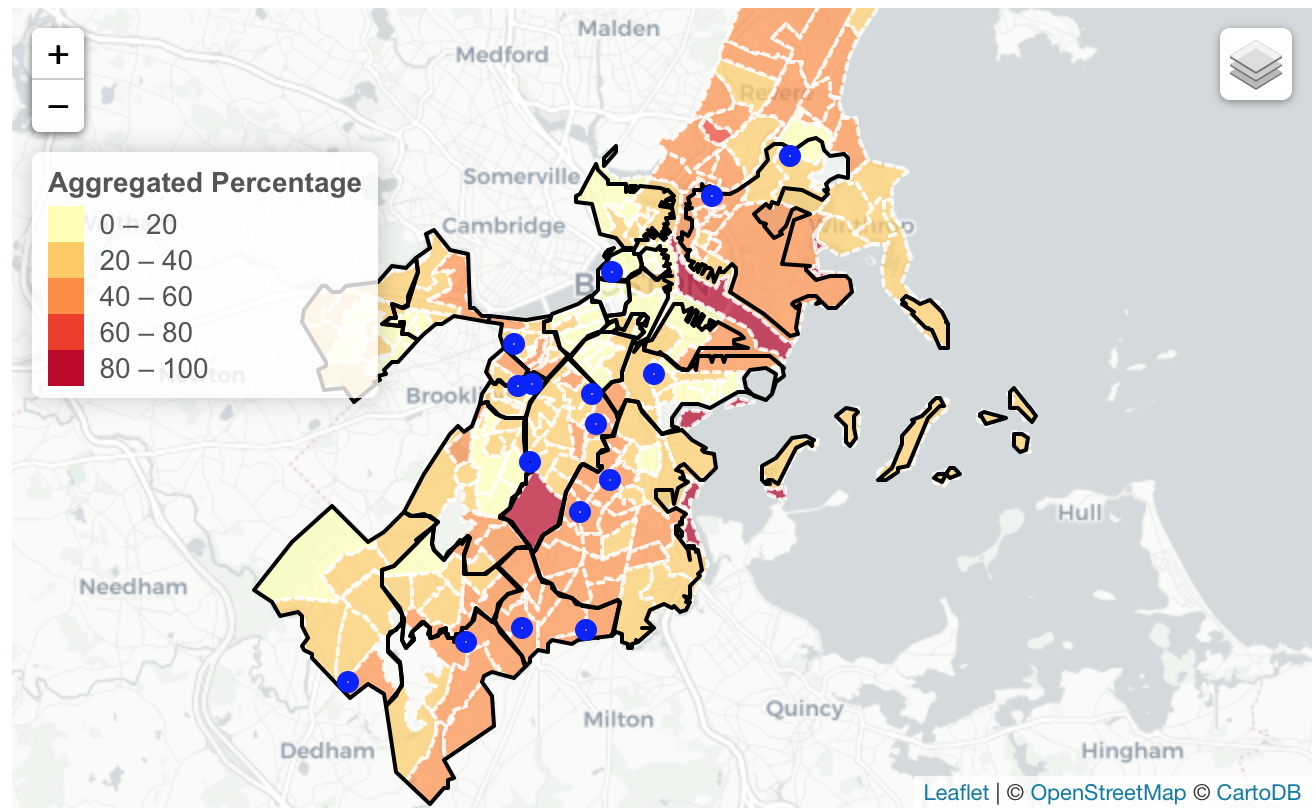
\includegraphics[width=0.8\linewidth]{aggregatehourdemand} 

}

\caption{Number of slots in certain tracts by providers who operate off hour during weekdays for early ed}\label{fig:unnamed-chunk-14}
\end{figure}

Figure 8 shows the aggregated percentage map of all people that work
nonstandard hours, which we create by adding the percentages found in
Figures 5 through 7. The blue dots represent providers that offer
nonstandard hour services for children under 6. This map indicates that,
generally, East Boston, downtown Boston, Roxbury, South Boston, and
waterfront areas are places where the largest amount of people have
nonstandard working schedules. However, we can see that there are only a
few providers that can take care of children from families in these
regions and these providers are located in the areas most in need of
off-hour early ed childcare services. There is no provider in the
Roxbury or waterfront areas at all. There is a significant lack of
irregular hour early ed childcare services across all areas.

\section{Challenges and Limitations}\label{challenges-and-limitations}

\subsection{Challenges}\label{challenges}

There are two main challenges that we faced this project. The first is
data cleaning of the EEC dataset. The EEC dataset has a messy data
format and a lot of columns that contain information on several
different variables. For example, to extract information that we need to
create the capacity and hours variables, we use various functions and
packages from R and Python to clean, merge, and spread several variables
from the original dataset, including minimum age, rates, open and close
time of providers that are composed of strings and special characters.

The second challenge is the geographical classification. One of the
narratives of this project is to look at the supply and demand by the
tract and neighborhood levels, the information of which are not provided
in the original datasets we are given. We dealt with this issue by
geocoding the providers' locations, deciding which polygon each provider
falls within using the over function from the rgeos package.

\subsection{Limitations}\label{limitations}

Our primary limitations in the dataset came from dealing with ACS data,
which entirely consists of estimates, as well as the issue of matching
variables from census dataset with those from EEC datasets.

First, census data in general consists entirely of estimates. This means
that there is inherently a margin of error in all the work that we
present, which is not present in any of the maps or tables primarily due
to time restraints. Secondly, some of the variables from census datasets
are based on assumptions different from real life situations, and the
focus of our project. Specifically, people's departure time for work is
created based on the assumption that people work for the same amount of
hours everyday while the parents we are most interested in are those
that have irregular working hours.

Second, our general lack of ability to match census data variables with
childcare provider variables when trying to quantify the same construct.
Although we successfully create the ratio of the number of children
under 6 from working families to the number of slots by using the
capacity and children population variables from the provider and census
datasets, there are many other variables that the project does not deal
with perfectly or could look into, such as income level of citizens
vs.~subsidy of providers. In addition, the percentage maps we create
based on people's departure time for works include all population while
our project actually focuses on working parents

Third, there is a lack of data in the EEC dataset about important
variables, such as the capacity of each provider by age groups and
subsidy amount in dollars. The absence of these variables prevents us
from looking more deeply into the supply for childcare services. There
are many variables that we clean but do not look into due to the limited
amount of time we have, such as subsidy, availability of drop-in and
emergency services.

\section{Discussion and Conclusion}\label{discussion-and-conclusion}

To examine the inconsistencies in the EEC by highlighting childcare
provision gaps in the Greater Boston Area, we use EEC datasets and
census datasets to create maps that illustrate a disparity in operating
hours and capacity for childcare providers on the neighborhood level and
census tract level. In a word, East Boston and West Boston
neighborhoods, including Allston, Boston, South Boston, Brighton,
Charlestown, Dorchester, East Boston, Hyde Park, Jamaica Plain,
Mattapan, Roslindale, Roxbury, and West Roxbury, are the regions where
the gaps apparently exist.

According to the visualizations of the ``capacity'' variable, providers
in East Boston and West Boston, where there is a large number of
children under 6, do not offer enough number of slots to feed the need
of families in these areas. Similarly, the maps on the ``hours''
variable indicate that there is a lack of childcare off hour services
for working families living in East Boston, West Boston, South Boston,
and the waterfront areas of Allston, Brighton, and Jamaica Plain are
most in need of off hour childcare services. According to the median
income level map of Boston, most of these neighborhoods are also regions
where income levels are lower than the average income level of the
Boston area {[}12{]}. The limited financial capability of citizens of
these areas might force them to work during irregular hours and to send
their children to the childcare providers. On the other hand, the
providers in these regions could not provide enough slots for children
under 6 as they could not earn as much money from these low-income
families as they could from families in the central areas. The policy
intervention and support from EEC could be urgent to resolve the gap.

In a word, our graphical analysis successfully illustrates the existence
of the gap between supply and demand for early ed childcare services in
the Greater Boston area. For researchers who are interested in digging
more deeply into this topic in the future, we suggest several directions
they could explore into. First, people could match more variables on the
demand for childcare services with variables on the supply for childcare
services to illustrate the existence of gaps. Second, people could try
to obtain a more comprehensive dataset from EEC to have a closer look at
the supply of childcare services for different age groups. Third, people
could conduct a childcare survey by themselves to have first-hand
information directly from the providers and families in need of
childcare services in Boston. Fourth, people could broaden our research
to look at Massachussetts as a whole. There is a lot more that could be
done in terms of researching the supply of childcare services, but the
current exploration could be a good starting point.

\section*{References}\label{references.unumbered}
\addcontentsline{toc}{section}{References}

\hypertarget{refs}{}
\hypertarget{ref-CLU}{}
1. Admin. Community labor united {[}Internet{]}. Community Labor United.
Community Labor United; 2019. Available: \url{http://massclu.org/}

\hypertarget{ref-duffy_albelda_hammonds_2013}{}
2. Duffy M, Albelda R, Hammonds C. Counting care work: The empirical and
policy applications of care theory. 2013; 1--23.
doi:\href{https://doi.org/129.64.99.141}{129.64.99.141}

\hypertarget{ref-EEC}{}
3. Weber TL. Department of early education and care {[}Internet{]}.
Mass.gov. Common Wealth of Massachusetts; 2019. Available:
\url{https://www.mass.gov/orgs/department-of-early-education-and-care}

\hypertarget{ref-epi_2015}{}
4. EPI. Irregular work scheduling and its consequences. Economic Policy
Institute Briefing Paper. 2015; 1--41. Available: \url{www.EPI.org}

\hypertarget{ref-lambert_henly_2014}{}
5. Lambert SJ, Henly JR. Measuring precarious work schedules. Employment
Instability, Family Well-Being, and Social Policy Network. 2014; 1--26.
Available: \url{www.ssascholars.uchicago.edu/einet}

\hypertarget{ref-adams_katz_2015}{}
6. Adams G, Katz M. Review of massachusetts child care subsidy
eligibility policies and practices. Urban Institute. 2015; 1--44.

\hypertarget{ref-bostonshapefile}{}
7. Harvard worldmap {[}Internet{]}. WorldMap. Available:
\url{http://worldmap.harvard.edu/data/geonode:boston_neighborhood_shapefiles_iq5}

\hypertarget{ref-R-tidyverse}{}
8. Wickham H. Tidyverse: Easily install and load the 'tidyverse'
{[}Internet{]}. 2017. Available:
\url{https://CRAN.R-project.org/package=tidyverse}

\hypertarget{ref-R-tigris}{}
9. Walker K. Tigris: Load census tiger/line shapefiles {[}Internet{]}.
2018. Available: \url{https://CRAN.R-project.org/package=tigris}

\hypertarget{ref-R-tidycensus}{}
10. Walker K. Tidycensus: Load us census boundary and attribute data as
'tidyverse' and 'sf'-ready data frames {[}Internet{]}. 2019. Available:
\url{https://CRAN.R-project.org/package=tidycensus}

\hypertarget{ref-childcare_desert}{}
11. Malik R, Hamm K, Schochet L, Novoa C, Workman S, Jessen-Howard S.
America's child care deserts in 2018 {[}Internet{]}. Center for American
Progress. Available:
\url{https://www.americanprogress.org/issues/early-childhood/reports/2018/12/06/461643/americas-child-care-deserts-2018/}

\hypertarget{ref-bostonmap}{}
12. Boston income map {[}Internet{]}. City-data. Available:
\url{http://www.city-data.com/income/income-Boston-Massachusetts.html}

\hypertarget{ref-R-base}{}
13. R Core Team. R: A language and environment for statistical computing
{[}Internet{]}. Vienna, Austria; 2017. Available:
\url{https://www.R-project.org/}

\hypertarget{ref-R-papaja}{}
14. Aust F, Barth M. papaja: Create APA manuscripts with R Markdown
{[}Internet{]}. 2018. Available: \url{https://github.com/crsh/papaja}

\hypertarget{ref-R-dplyr}{}
15. Wickham H, François R, Henry L, Müller K. Dplyr: A grammar of data
manipulation {[}Internet{]}. 2019. Available:
\url{https://CRAN.R-project.org/package=dplyr}

\hypertarget{ref-R-forcats}{}
16. Wickham H. Forcats: Tools for working with categorical variables
(factors) {[}Internet{]}. 2018. Available:
\url{https://CRAN.R-project.org/package=forcats}

\hypertarget{ref-R-ggformula}{}
17. Kaplan D, Pruim R. Ggformula: Formula interface to the grammar of
graphics {[}Internet{]}. 2017. Available:
\url{https://CRAN.R-project.org/package=ggformula}

\hypertarget{ref-R-ggplot2}{}
18. Wickham H. Ggplot2: Elegant graphics for data analysis
{[}Internet{]}. Springer-Verlag New York; 2016. Available:
\url{https://ggplot2.tidyverse.org}

\hypertarget{ref-R-lattice}{}
19. Sarkar D. Lattice: Multivariate data visualization with r
{[}Internet{]}. New York: Springer; 2008. Available:
\url{http://lmdvr.r-forge.r-project.org}

\hypertarget{ref-R-leaflet}{}
20. Cheng J, Karambelkar B, Xie Y. Leaflet: Create interactive web maps
with the javascript 'leaflet' library {[}Internet{]}. 2018. Available:
\url{https://CRAN.R-project.org/package=leaflet}

\hypertarget{ref-R-leaflet.extras}{}
21. Karambelkar B, Schloerke B. Leaflet.extras: Extra functionality for
'leaflet' package {[}Internet{]}. 2018. Available:
\url{https://CRAN.R-project.org/package=leaflet.extras}

\hypertarget{ref-R-mapview}{}
22. Appelhans T, Detsch F, Reudenbach C, Woellauer S. Mapview:
Interactive viewing of spatial data in r {[}Internet{]}. 2018.
Available: \url{https://CRAN.R-project.org/package=mapview}

\hypertarget{ref-R-Matrix}{}
23. Bates D, Maechler M. Matrix: Sparse and dense matrix classes and
methods {[}Internet{]}. 2017. Available:
\url{https://CRAN.R-project.org/package=Matrix}

\hypertarget{ref-R-mosaic}{}
24. Pruim R, Kaplan DT, Horton NJ. The mosaic package: Helping students
to 'think with data' using r. The R Journal. 2017;9: 77--102. Available:
\url{https://journal.r-project.org/archive/2017/RJ-2017-024/index.html}

\hypertarget{ref-R-mosaicData}{}
25. Pruim R, Kaplan D, Horton N. MosaicData: Project mosaic data sets
{[}Internet{]}. 2016. Available:
\url{https://CRAN.R-project.org/package=mosaicData}

\hypertarget{ref-R-purrr}{}
26. Henry L, Wickham H. Purrr: Functional programming tools
{[}Internet{]}. 2019. Available:
\url{https://CRAN.R-project.org/package=purrr}

\hypertarget{ref-R-readr}{}
27. Wickham H, Hester J, Francois R. Readr: Read rectangular text data
{[}Internet{]}. 2017. Available:
\url{https://CRAN.R-project.org/package=readr}

\hypertarget{ref-R-sf}{}
28. Pebesma E. Simple Features for R: Standardized Support for Spatial
Vector Data. The R Journal. 2018; Available:
\url{https://journal.r-project.org/archive/2018/RJ-2018-009/index.html}

\hypertarget{ref-R-stringr}{}
29. Wickham H. Stringr: Simple, consistent wrappers for common string
operations {[}Internet{]}. 2019. Available:
\url{https://CRAN.R-project.org/package=stringr}

\hypertarget{ref-R-tibble}{}
30. Müller K, Wickham H. Tibble: Simple data frames {[}Internet{]}.
2019. Available: \url{https://CRAN.R-project.org/package=tibble}

\nolinenumbers


\end{document}

